\documentclass[12pt]{article}
\usepackage[a4paper, total={6in, 8in}, margin=1in]{geometry}
\usepackage[style=bath,sorting=ynt]{biblatex}
\usepackage{lmodern}
\usepackage{parskip}
\usepackage{amsmath}
\usepackage{titlesec}
\usepackage{caption}
\usepackage{float}
\usepackage[table,x11names]{xcolor}
\setcounter{secnumdepth}{4}
\usepackage{pgfgantt}
\usepackage{lscape}
\usepackage{graphicx}
\graphicspath{ {./images/} }

\addbibresource{References.bib}

\begin{document}
%==================================
%	TITLE PAGE
%==================================
\begin{titlepage}
	\begin{center}
		\vspace*{1cm}
		
		Imperial College London \\
		Department of Earth Science and Engineering \\
		MSc in Applied Computational Science and Engineering
		
		\vspace{1cm}
		
		Independent Research Project \\
		Project Plan
		
		
		\vspace{1cm}
		
		
		{\fontsize{18}{104}\selectfont \textbf{ CoNuS-Viz: A Visualization Package for the Concurrent Library for Numerical Simulations}}

		
		\vspace{1cm}
		
		by \\ 
		Fazal Khan
		
		\vspace{1cm}
		
		Supervisor: \\
		Professor Cédric John
		
		\vspace{1cm}
		
		Email: \\
		fk4517@ic.ac.uk
		
		\vspace{1cm}
		
		GitHub login: \\
		acse-fk4517
		
		\vspace{1.0cm}
		
		June 2020
		
	\end{center}
\end{titlepage}	
%==================================
%	Introduction
%==================================
\section{Introduction}

\subsection{Forward Modelling}

Many natural or social phenomena such as fluid-flow or population dynamics may be formulated as a model that evolves with time. Formulating a process this way allows it to be simulated using computational techniques. Suppose $\vec y$ denotes the variables of interest stored in a vector, then a general forward model describing their evolution with respect to time can be written as:

\begin{center}
	\begin{equation}
	\vec y_{t+1} = f(t, ~\vec y_t)
	\end{equation}
\end{center}

From this we can see that in order to update the variables of interest, $\vec y_t$, we must consider both time, $t$ and the previous state of the variables of interest, $\vec y_{t-1}$.

As mentioned, this general technique can be applied in many different fields. As a concrete example consider one such field known as Stratigraphy. Stratigraphy is concerned with the processes which lead to the organization of rocks in space and time. Stratigraphic Forward Models (SFM) are forward models which have been used to simulate realistic stratigraphic processes based on a set of reasonable geologic parameter values. These parameters may consist of items such as tectonic movement and erosion \autocite{10.2110/pec.99.62.0069}.

When studying stratigraphic observational data, it is often important to understand what set of initial geological conditions may have caused the stratigraphic patterns in the observations. Problems of this type can be generally classified as inverse problems \autocite{10.1260/0144598011492363}. SFMs can be used to generate a set of outputs which in turn are compared to observations. Outputs are generated systematically for a range of initial parameter values, and those outputs which are close to the observations within a pre-defined bound are then taken as solutions to this inverse problem. Used in this way SFMs are an integral part of solving inversion problems in stratigraphy. More generally, solving inverse problems in this way can be useful for many other domains ranging from finance to physics.

\subsection{Computational Intensity of Large Forward Models}
Large forward models are computationally intensive methods which may require generating many outputs to find a satisfactory solution. For example in order to solve inverse problems, not only are many outputs generated, but the set of input geological parameters, $\vec y_i$ is often also very large too \autocite{10.1260/0144598011492363}.

For these reasons computational techniques that can deal with large models efficiently are very important in practice. One way to address this is to use concurrency and parallelism when performing calculations on the underlying data. Such techniques have been used in scientific modelling for increasing performance and reducing computation time. Domains ranging from biophysical modelling to computational fluid dynamics have benefited from technologies such as GPUs that allows these techniques to be more readily exploited \autocite{4490127}.

\subsection{The Concurrent Library for Numerical Simulations (CoNuS)}
CoNuS is an experimental open-source library developed by Professor Cédric John from the Carbonate Research Group at Imperial College London. The library is written in the Scala programming language and has two general aims:

\begin{enumerate}
\item \textbf{Abstraction}: Abstract away unnecessary implementation details from the user so they can focus on the modelling. \\
\item \textbf{Performance}: Be performant enough to run large, concurrent models in a reasonable amount of time.
\end{enumerate}

\subsubsection{Abstraction}
Conventional forward models generally require users to define a grid of variables, some type of mathematical equation that defines how variables evolve with time, and a loop to actually carry out calculations. CoNuS abstracts away these common mechanics of forward models so that users from any discipline, regardless of their programming experience, can compose models by focusing on the mathematical basis for how variables evolve. Users essentially define equation (1), and let the model run.

\subsubsection{Performance}
CoNuS leverages the Scala programming language and functional programming techniques to enhance performance and program correctness. Functional programming techniques are excellent at creating data recursion schemes that can exploit concurrency and parallelism; an example is Google's famous MapReduce algorithm which processes large datasets in parallel \autocite{LAMMEL20081}. 

Since it is written in Scala, CoNuS benefits from several language features that make writing concurrent code easier. Scala is a statically typed, compiled language that targets the Java Virtual Machine (JVM) \autocite{scala}. A strong type system can be very useful in designing software as it allows a programmer to discover variants and trigger generalizations that simplify design \autocite{LAMMEL20081}. 

Scala also combines both object-orientated and functional programming concepts to create highly expressive programs that can support many levels of abstraction over the underlying computation. One such abstraction is the Scala actor model which allows concurrent code to be written ergonomically in a type-safe manner. The actor model was introduced to deal with the JVMs shared-memory thread model, which suffered from high memory consumption and context switching costs \autocite{haller_odersky_2009}. The Scala actors library has since been deprecated and replaced by the Akka library, which is built on the same concept and allows code to be run on clusters \autocite{akka}. Making use of actors on clusters is on the roadmap for the CoNuS library.

\section{Project Aims}
As CoNuS is experimental, it currently lacks an integrated visualization library. The aim of this independent research project will be to design and build a visualization library with the following aims:

\begin{itemize}
\item Create an easy-to-use, general purpose plotting library for Scala that can plot scientific data, much like matplotlib for Python \autocite{matplotlib}.
\item Allow CoNuS forward models to be visualized.
\item Implement enhanced functionality that creates interactive scientific charts, not just static ones. 
\item Integrate the library to run seamlessly with Jupyter notebooks, in addition to running on the JVM.
\item Leverage functional programming design and Scala's type system to ensure program correctness.
\item Make an original contribution to the Scala open-source community.
\end{itemize}

\subsection{Schedule}
In this section I will outline the expected project schedule. Some of the items in the schedule were already underway or completed as of the time of writing.

\subsubsection{Phase 1: Preparation}

\textbf{i. Literature Review}

I will review literature on forward modelling, data visualization and functional programming techniques. 

At the time of writing, I have completed the literature review on forward modelling, understand why the CoNuS library exists, and why there is the need to develop a visualization library for it. I will continue to read more articles on data visualization and functional programming techniques. \\

\textbf{ii. Review Existing Visualization Libraries}

At the time of writing I have reviewed existing visualization libraries for Scala and the JVM. I have concluded that non of the existing options meet the requirements for this project. After looking at the rich Javascript open-source ecosystem, I have decided to leverage the Plotlyjs library as the basis for this project. \\

\textbf{iii. Learn Functional Programming Techniques}

This will consist of reviewing functional approaches to designing software, understanding Scala's type system and how to utilize Scala's functional features to build robust software. \\

\textbf{iv. Implement Basic Library Structure}

At the time of writing I have implemented basic code for rendering charts. I will expand on this by adding more visualization options and additional interactive chart components as they are required. \\

\textbf{v. Write Project Plan}

I will begin writing the project plan ready for submission by the 25th of June.

\subsubsection{Phase 2: Execution}

\textbf{i. Design Advanced Components of Library}

This will consist of building on the existing code I wrote in the previous phase. This may require refactoring of the library and making it more structured by using interfaces and abstracting out redundant code. I will also try and make the code more efficient if required. \\

\textbf{ii. Review Best Practices}

Here I will review more closely work done with existing state-of-the-art visualization libraries. This will ensure that the existing codebase is in line with best practices. \\

\textbf{iii. Write Summary of Work Done So Far}

I will maintain notes on the work done so far, with the aim of combining these notes into a single document for my independent research project report. \\

\textbf{iv. Review Codebase}

Review the codebase and remove redundant or inefficient code. 

\subsubsection{Phase 3: Summary}

\textbf{i. Test Library}

Run full suite of unit tests and get the codebase to compile and pass all the tests. In addition, test the library from a user's perspective by creating an example notebook in Jupyter making full use of library functionality. Make any final changes to codebase. \\

\textbf{ii. Write Independent Research Report}

Combine all the summaries into one coherent document and write the Independent Research Report. \\

\section{Risks and Mitigation}

The main risk is being unable to make progress quickly enough before the deadline due to the complexity of the Scala type system. To mitigate this risk I will create my library incrementally and in a modular manner. This will ensure that even if I run out of time, the library will still have some basic visualization capabilities even if incomplete.

\pagebreak
\begin{landscape}
	
\begin{figure}[h]
\begin{center}
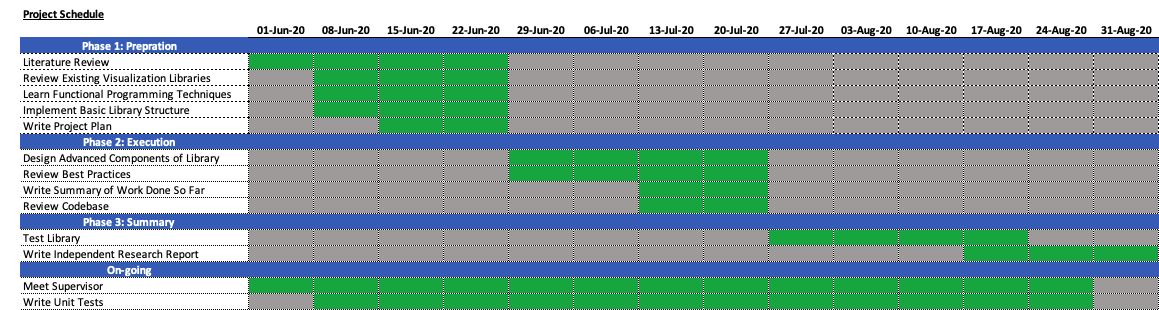
\includegraphics[scale=0.65]{Gantt}
\end{center}
\caption{Gantt Chart of Expected Project Schedule}
\end{figure}

\end{landscape}
\pagebreak
\printbibliography

\end{document}